\chapter{Stage}
\label{ch:tesi:stage}

\section{Piano di stage}
\label{sec:tesi:stage:piano}

\subsection{Obiettivi e requisiti}
\label{sec:tesi:stage:piano:obiettivi}
L'attività di stage si colloca nell'ambito del progetto presentato nel capitolo \ref{ch:tesi:progetto} e persegue due obiettivi distinti ma correlati, focalizzandosi sulla componente \textit{social} della piattaforma.

\paragraph{Criteri di classificazione}
Il primo obiettivo consiste nell'estendere l'attuale sistema di classificazione (v. sezione \ref{sec:tesi:progetto:classificazione}) integrandovi un criterio aggiuntivo per la catalogazione dei contenuti pubblicati dagli utenti e la costruzione di un'enciclopedia della conoscenza per rendere il reperimento e la consultazione delle informazioni desiderate il più efficiente ed agevole possibile.

L'ideazione e concezione del suddetto criterio deve tener conto della natura tematica della piattaforma, riuscendo a conciliare due esigenze distinte:
\begin{itemize}
\item dev'essere sufficientemente astratto e flessibile per adattarsi alla molteplicità di varianti tematiche in cui la piattaforma stessa può essere declinata;
\item dev'essere ottimizzato per avvantaggiarsi delle peculiarità di una piattaforma tematica, ad esempio la maggior correlazione degli argomenti trattati.
\end{itemize}

La soluzione individuata deve inoltre prescindere da assunzioni legate alla tecnologia utilizzata. Infine, alla luce di possibili evoluzioni nello sviluppo della piattaforma, si desidera che la classificazione di un contenuto informativo (assegnazione di metadati, individuazione di correlazioni, \ldots) possa essere - in futuro - demandata a componenti software integrate nella piattaforma.

\paragraph{Interfaccia grafica}
Il secondo obiettivo consiste nel progettare un'interfaccia grafica per la consultazione dei contenuti informativi, che sfrutti il criterio di classificazione aggiuntivo per facilitare la ricerca ed il reperimento delle informazioni di interesse per l'utente all'interno del patrimonio enciclopedico della piattaforma. La sfida principale consiste nel progettare un'interfaccia in grado di visualizzare in maniera chiara e ordinata un ridotto o elevato numero di contenuti, a prescindere dalla classe del dispositivo impiegato (\textit{smartphone}, \textit{tablet}, \textit{notebook}, \ldots).

Il primo passo consiste nell'individuare le informazioni essenziali ad una rapida e precisa identificazione dei contenuti (titolo, autore, data, \ldots) e valutare la notazione (grafica o testuale) più adatta per esprimerle, al fine di renderle accessibili al maggior numero possibile di utenti; le informazioni aggiuntive devono essere comunque accessibili, ma solo su esplicita richiesta dell'utente. In questo ambito si inseriscono una serie di analisi e valutazioni di carattere sociologico, svolte da altri membri del team di progetto, per individuare le soluzioni più idonee a comunicare tali informazioni in modo da renderne la comprensione chiara e intuitiva a qualsiasi utente.

Il secondo passo richiede di definire le specifiche per un'interfaccia facilmente navigabile, che sia in grado di mostrare in modo ordinato e intuitivo i contenuti e le reciproche relazioni. Occorre perciò individuare opportuni criteri di raggruppamento, ordinamento e collocamento dei contenuti visualizzati per favorirne la consultazione, evitando un sovraccarico cognitivo e garantendo un livello adeguato di leggibilità.

Con il terzo ed ultimo passo si intende aggiungere la possibilità per l'utente di filtrare i contenuti visualizzati in accordo a proprietà (argomento, autore, data di pubblicazione, tipo) o metadati associati (attinenza, emozioni, giudizi, intenzioni). Per gli utenti autenticati si desidera offrire un livello aggiuntivo di personalizzazione, che consenta di filtrare automaticamente i contenuti secondo le preferenze associate al profilo (interessi, livello di esperienza).

Per individuare i requisiti essenziali si prendono innanzi tutto in considerazione alcuni casi d'uso classici:
\begin{enumerate}
\item l'utente naviga liberamente tra i contenuti (più recenti, più letti, più discussi, \ldots);
\item l'utente consulta la discussione generata da un singolo contenuto;
\item l'utente cerca le informazioni riguardanti un certo tema (contenuti affini, \ldots);
\item l'utente esplora gli argomenti trattati e le reciproche relazioni.
\end{enumerate}

\subsection{Pianificazione}
L'attività di stage viene suddivisa in due fasi distinte per semplificarne la pianificazione:
\begin{enumerate}
\item l'estensione del sistema di classificazione;
\item l'analisi e la progettazione dell'interfaccia grafica.
\end{enumerate}

Per ciascuna fase sono fissati gli obiettivi generali, sono individuate e organizzate su base settimanale le attività da svolgere, cercando di garantire un carico di lavoro equilibrato, e sono indicati i prodotti attesi. La durata complessiva dello stage si attesta su 8 settimane a tempo pieno, corrispondenti a 320 ore di lavoro.

\begin{table}[ht]
\centering
\begin{tabular}{|p{10cm}|c|}
\hline
\textsc{Attività} & \textsc{Ore di lavoro} \\ \hline
\multicolumn{2}{|c|}{\textit{Fase 1: estensione del sistema di classificazione}} \\ \hline 
Analisi delle specifiche del sistema di classificazione & 40 \\ \hline
Analisi comparativa dei principali sistemi di classificazione della conoscenza & 40 \\ \hline
Progettazione del sistema di classificazione & 40 \\ \hline
Implementazione del sistema di classificazione nel modello relazionale & 40 \\ \hline
\multicolumn{2}{|c|}{\textit{Fase 2: analisi e progettazione dell'interfaccia grafica}} \\ \hline 
Analisi dei requisiti dell'interfaccia grafica & 40 \\ \hline
Progettazione dell'interfaccia grafica: visualizzazione dei contenuti & 40 \\ \hline
Progettazione dell'interfaccia grafica: filtraggio dei contenuti & 40 \\ \hline
Progettazione dell'interfaccia grafica: navigazione dei contenuti & 40 \\ \hline
\end{tabular}
\caption{Pianificazione settimanale delle attività}
\label{tab:tesi:stage:pianificazione}
\end{table}

\begin{figure}[ht]
\begin{center}
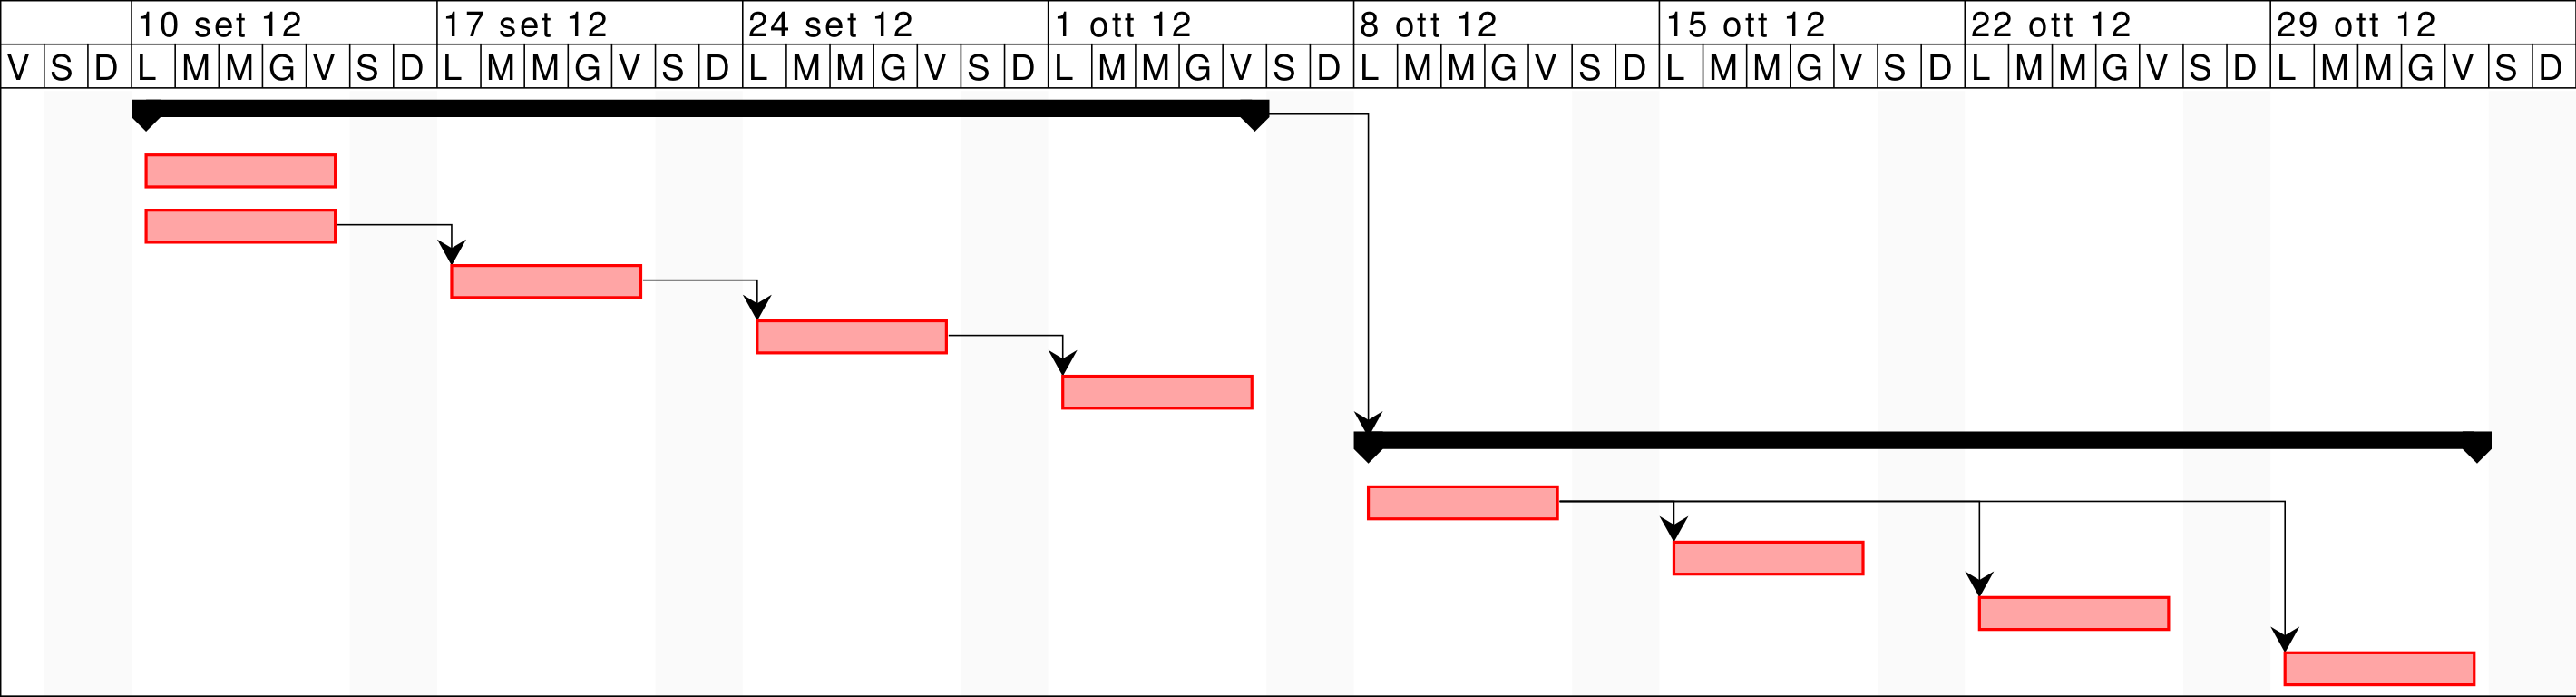
\includegraphics[width=14.5cm]{gantt.png}
\label{fig:tesi:stage:gantt}
\caption{Diagramma di Gantt}
\end{center}
\end{figure}

\section{Norme di stage}

\paragraph{Ambiente di lavoro}
Nel corso dello stage sono stati impiegati diversi strumenti per gestire le attività di progetto e produrre la documentazione prevista.

\begin{table}[ht]
\centering
\begin{tabular}{|l|l|}
\hline
\textsc{Controllo di versione} & \underline{Mercurial} 2.0.2 \\ \hline
\textsc{Editor \LaTeX} & \underline{LaTeXila} 2.4.0 - \underline{gedit} 3.4.0 con \textit{gedit-latex-plugin} \\ \hline
\textsc{Editor UML} & \underline{UMLet} 11.5.1 \\ \hline
\textsc{Foglio elettronico} & \underline{LibreOffice Calc} 3.6 \\ \hline
\textsc{Gestione database} & \underline{MySQL Workbench} 5.2.42 \\ \hline
\textsc{Mockup} & \underline{Pencil} 2.0.2 \\	\hline
\textsc{Pianificazione} & \underline{ProjectLibre} 1.5.1 \\ \hline
\textsc{Repository} & \underline{Bitbucket} \\ \hline
\textsc{Sistema operativo} & \underline{Ubuntu} 12.04 \\ \hline
\end{tabular}
\caption{Configurazione dell'ambiente di lavoro}
\label{tab:tesi:stage:norme:strumenti}
\end{table}

\paragraph{Documentazione}
La documentazione è stata redatta in \LaTeX\ e pubblicata in formato \underline{PDF}. A ciascun documento è assegnato un numero di versione $x.y$, ove $x$ rappresenta l'ultima \textsc{versione formale}, rivista e approvata dal referente aziendale e disponibile a terze parti interessate (membri del team di progetto, tutor interno), mentre il numero $y$ si riferisce ad una \textsc{versione preliminare} per uso interno, eventualmente consultabile dal referente aziendale.

\paragraph{Modello relazionale}
Il modello relazionale del database è stato realizzato mediante lo strumento adottato dal team di progetto, ossia l'editor \textit{MySQL Workbench}, per facilitare la condivisione e l'integrazione delle informazioni.

I nomi delle tabelle sono espressi in lingua italiana e contengono solo caratteri alfabetici minuscoli e non accentati, eventualmente separati mediante il simbolo '\textunderscore' (trattino basso). I nomi degli attributi, preceduti dal nome della tabella e dal carattere '.' (punto), sono espressi in lingua italiana e contengono solo caratteri alfabetici in formato \underline{CamelCase}, ove la lettera iniziale è sempre in minuscolo.

\paragraph{Digrammi UML}
Durante l'attività di stage sono stati redatti e inclusi nella documentazione diversi diagrammi \underline{UML} dei casi d'uso, dei package e delle classi, di cui sono presenti svariati esempi nel prosieguo del documento.

I nomi delle sottoclassi riportano per esteso o in forma abbreviata l'identificatore della superclasse diretta: nel secondo caso sono presenti - come prefisso - le sole lettere maiuscole, nel medesimo ordine di apparizione.

\paragraph{Casi d'uso}
La notazione utilizzata per identificare un caso d'uso è così definita:
$$UC.x.y$$
ove:
\begin{itemize}
\item $UC$ è l'abbreviazione di \textit{Use Case} (Caso d'uso);
\item $x \in \left\{1,2,\ldots\right\}$ è il numero identificativo del diagramma cui appartiene il caso d'uso;
\item $y \in \left\{1,2,\ldots\right\}$ è il numero associato al caso d'uso.
\end{itemize}

\paragraph{Requisiti funzionali}
I requisiti del sistema software sono univocamente identificati mediante la seguente notazione:
$$Rf.x.y$$
ove:
\begin{itemize}
\item $Rf$ è l'abbreviazione di \textit{requisito funzionale};
\item $x \in \left\{ob,de\right\}$ rappresenta il tipo di requisito funzionale (\textit{ob} per obbligatorio, \textit{de} per desiderabili);
\item $y \in \left\{1,2,\ldots\right\}$ è il numero associato ad un requisito.
\end{itemize}

\paragraph{Tracciamento dei casi d'uso}
Il tracciamento delle dipendenze tra casi d'uso e requisiti software è stato realizzato mediante un foglio elettronico, ove:
\begin{itemize}
\item ciascuna riga rappresenta un requisito del sistema software;
\item ciascuna colonna rappresenta un caso d'uso;
\item ciascuna cella contiene il carattere 'X' se esiste una relazione di dipendenza tra il caso d'uso e il requisito, altrimenti è vuota.
\end{itemize}

Per ciascuna riga e colonna viene impiegata una semplice formula per asserire la completezza e la necessità della matrice dei requisiti:  
\begin{center}
\texttt{CONTA.SE(A:Z;``X'')}   
\end{center}
ove:
\begin{itemize}
\item \texttt{A:Z} corrisponde all'intervallo di celle di una singola riga o colonna;
\item \texttt{"X"} rappresenta il pattern da cercare;
\item \texttt{CONTA.SE} è una funzione che accetta due argomenti (l'intervallo di celle ed il \textit{pattern}) e restituisce il numero di celle appartenenti all'intervallo contenenti una o più occorrenze del \textit{pattern} specificato.
\end{itemize}

\paragraph{Completezza} Per ogni colonna, se la formula restituisce un valore pari a 0 (zero) sta ad indicare che il requisito utente non è soddisfatto da alcun requisito software.

\paragraph{Necessità} Per ogni riga, se la formula restituisce un valore pari a 0 (zero) sta ad indicare che il requisito software corrispondente è superfluo.

%--------
% SECTION
%--------
\section{Criterio di classificazione}
\label{sec:tesi:stage:criterio-classificazione}
Il patrimonio di conoscenza della piattaforma è garantito essenzialmente dai contenuti pubblicati dagli utenti ed arricchito dal loro valore informativo: ciascuno di essi, a prescindere dalla forma (testo, immagini, audio, video, \ldots) o dalla classe (domanda, discorso, evento, recensione, \ldots), condivide delle informazioni inerenti uno o più elementi del dominio tematico della piattaforma.

\begin{figure}[ht]
\begin{center}
 
\includegraphics{placeholder.png}
 \label{fig:tesi:stage:classificazione:serbatoio-contenuti}
 \caption{Valore informativo di un contenuto}
\end{center}
\end{figure}

\subsection{Enciclopedia del sapere}
\label{sec:tesi:stage:criterio-classificazione:enciclopedia}
Attualmente, il limite della piattaforma consiste nell'essere un serbatoio di \textsc{contenuti informativi} disaggregati e priva degli strumenti per classificare e catalogare il sapere custodito conferendovi una struttura ordinata, una sorta di indice in grado di facilitarne la ricerca, il reperimento e la consultazione.

L'obiettivo del criterio di classificazione consiste essenzialmente nel costruire un'enciclopedia del sapere a partire dalle informazioni presenti nei contenuti informativi.

\begin{quotation}
Un'enciclopedia è un'opera letteraria che raccoglie e ordina la sintesi della conoscenza umana in tutti i campi o in un determinato settore. Le enciclopedie sono divise in voci, o lemmi, cui si accede di solito in ordine alfabetico.
\begin{center}[\ldots]\end{center}
Le enciclopedie possono essere generali, e contenere voci su qualsiasi argomento (lettere, scienze, arti), oppure specialistiche e concentrarsi su un particolare campo della conoscenza (ad esempio un'enciclopedia di medicina o di filosofia). \cite{wiki:enciclopedia}
\end{quotation}

Il modello concettuale dell'enciclopedia diventa un riferimento utile ad identificare:
\begin{enumerate}
	\item i casi d'uso essenziali concernenti la consultazione del sapere custodito nella piattaforma (ricerca per lemma, argomento o affinità);
	\item gli elementi strutturali del sistema di classificazione (lemmi, accezioni, \ldots);
	\item i requisiti e le specifiche più rilevanti per il criterio di classificazione;
	\item le principali criticità rispetto alla coerenza e consistenza dell'enciclopedia.
\end{enumerate}

\paragraph{Contenuto informativo}
Ciascun contenuto può essere considerato una collezione di frammenti di informazioni, che contribuiscono ad arricchire la conoscenza relativa ad uno o più lemmi dell'enciclopedia: il criterio di classificazione deve quindi tenere traccia della relazione tra contenuti informativi e lemmi per essere in grado di catalogare e ricostruire l'intera conoscenza disponibile riguardo un certo tema.

\paragraph{Entità}
Nell'ambito della piattaforma, i lemmi vengono definiti \textsc{entità} ($d_i \in D$) e rappresentano elementi concreti (luoghi, persone, eventi, \ldots) o astratti (concetti, temi, \ldots) a cui afferiscono i contenuti. L'insieme delle entità definite - in un certo istante - all'interno della piattaforma rappresenta il \textsc{dominio della conoscenza} (di seguito per brevità \textsc{dominio}).

\begin{figure}[ht]
	\begin{center}
		
\includegraphics{placeholder.png}
		\label{fig:tesi:stage:fase-uno:entita-relazioni}
		\caption{Relazioni tra le entità del dominio}
	\end{center}
\end{figure}

Così come ciascun lemma di un'enciclopedia contiene spesso riferimenti ad altre voci, che trattano temi specifici o attinenti, nella piattaforma ciascuna entità può riferire o essere riferita da un numero arbitrario di entità distinte e possono esistere riferimenti incrociati, ossia coppie di entità che si citano a vicenda.

Ciò si traduce nel modello relazionale con un vincolo referenziale di tipo molti-a-molti tra le entità, che distingue entità referenti e riferite e permette così di interpretare il dominio $D$ come una struttura a grafo orientato ove:
\begin{itemize}
\item ciascun nodo rappresenta un entità;
\item ciascun arco uscente identifica un'entità riferita;
\item ciascun arco uscente identifica un'entità referente.
\end{itemize}

\paragraph{Etichette}
Ciascuna entità ha un valore semantico preciso ed univoco, ma dev'essere identificata anche sul piano sintattico mediante un'\textsc{etichetta} ($e_j \in E$), ossia una stringa di lunghezza variabile che consenta agli utenti di riferirla all'interno di ciascun contenuto. L'insieme di etichette definite in un certo istante costituisce il \textsc{dizionario} $E$ della piattaforma.

Il modello illustrato presenta tuttavia due notevoli inconvenienti, che devono essere risolti per soddisfare i requisiti e gli obiettivi previsti per il criterio di classificazione: l'ambiguità sintattica e quella semantica.

\subsection{Ambiguità sintattica}
\label{sec:tesi:stage:criterio-classificazione_ambiguità-sintattica}
Nel linguaggio comune, è possibile riferirsi ad una certa entità ($d_i$) con termini o espressioni differenti ($e_{i,j} \in E_i$): la presenza di sinonimi, aventi il medesimo valore semantico ma diversa sintassi, rappresenta un fattore di ambiguità intrinseco e non trascurabile, che trasforma la relazione uno-a-uno tra entità ed etichette in una di tipo uno-a-molti.

\begin{figure}[ht]
	\begin{center}
		
\includegraphics{placeholder.png}
		\label{fig:tesi:stage:fase-uno:ambiguita-sintattica}
		\caption{Ambiguità sintattica di un'entità (+ modello relazionale)}
	\end{center}
\end{figure}

Il criterio di classificazione è dunque chiamato a conciliare la possibilità per l'utente di riferirsi ad una certa entità con etichette differenti e l'esigenza di identificarla univocamente nei contenuti informativi.

\paragraph{Sinonimi}
La gestione dei sinonimi di un'entità rappresenta un aspetto cruciale, poiché scegliere tra i possibili sinonimi un'etichetta arbitraria con cui identificare un'entità ed ignorare i rimanenti, pur semplificando il modello, costringerebbe gli utenti a conoscere e ad utilizzare solo quell'etichetta imponendo una scelta del tutto arbitraria e - in quanto tale - fortemente soggettiva.

Per facilitare la ricerca di un'entità è opportuno includere e conservare nel dizionario tutte le etichette note o utilizzate dagli utenti, così da rendere il sistema sempre più accurato nell'individuare e riconoscere l'entità cui un utente fa riferimento quando utilizza una certa etichetta. Con il passare del tempo, il numero dei sinonimi di ciascuna entità è destinato a crescere grazie al contributo degli utenti, garantendo così una migliore copertura sintattica.

La proliferazione di sinonimi, ossia etichette equivalenti sul piano semantico ma sintatticamente differenti, rischia tuttavia di avere pesanti ripercussioni sull'efficacia del criterio di classificazione e particolarmente sull'efficienza della ricerca: se ai contenuti vengono assegnate delle etichette, reperire tutte e sole le informazioni inerenti una certa entità richiederebbe infatti di cercare riscontri nei contenuti pubblicati per ogni etichetta con cui possa venir riferita.

\paragraph{Contenuti}
A tale inconveniente si pone rimedio facilmente definendo una relazione molti-a-molti tra le entità e i contenuti, che ignori le etichette utilizzate per indicarle: così facendo si preserva l'identificazione univoca di ciascuna entità nei contenuti informativi, almeno sul piano semantico, e si guadagna in termini di efficienza.

Si considerino il dizionario $E$ ed il dominio $D$. Il numero medio $\alpha$ di etichette associato a ciascuna entità è pari a:
\begin{equation} \label{eq:tesi:stage:etichette-per-entità}
\alpha = \frac{\left|E_0\right| + \left|E_1\right| + \ldots}{\left|D\right|} = \frac{\sum{\left|E_i\right|}}{\left|D\right|}
\end{equation}
ove
\begin{equation} \label{eq:tesi:stage:dizionario}
\sum{\left|E_i\right|} = \left|E\right| \: \footnote{Poiché la relazione tra etichette ed entità è di tipo uno-a-molti, ciascuna etichetta è associata ad una ed una sola entità. Ne consegue che $P = {E_0, E_1, \ldots}$ è una partizione di $E$, ossia vale $\bigcup E_i = E$ e $\forall A \in P, B \in P: A \neq B \implies A \cap B = \emptyset$.}
\end{equation}

Ciò significa intuitivamente che assegnare ai contenuti un'etichetta arbitraria aumenterebbe di una costante moltiplicativa $\alpha$ la complessità dell'operazione ricerca, che dovrebbe essere ripetuta per ciascuna delle $\alpha$ etichette anziché per la sola entità corrispondente.\footnote{Si assuma per semplicità che la ricerca verifichi - per ciascun contenuto - quali termini cercati (entità o etichette) siano presenti, uno per volta, e che la complessità computazionale sia equivalente in entrambi i casi.}

\paragraph{Etichette}
Tuttavia, per riferire un'entità nella piattaforma web occorre caratterizzarla anche sul piano sintattico: sebbene non vi siano particolari controindicazioni nel permettere all'utente di scegliere l'etichetta da utilizzare nei contenuti che pubblica, si rischia di:
\begin{itemize}
	\item generare ambiguità e confusione tra gli utenti stessi, rendendo poco intuitivo stabilire se due entità citate in due contenuti diversi e con etichette differenti siano effettivamente la stessa;
	\item dover aggiungere alla relazione tra entità e contenuti un informazione aggiuntiva, ossia l'etichetta scelta per indicarla.
\end{itemize}

Per tale ragione, si individua arbitrariamente - per ciascuna entità $d_i$ - un'\textsc{etichetta primaria} ($e_{i,0} \in E_i$), che la identifica univocamente nell'ambito della piattaforma, mentre le restanti (\textsc{etichette secondarie}) ne vengono considerate sinonimi.

Così facendo si introducono tuttavia alcuni vincoli aggiuntivi sulla relazione, che risulta scissa in due distinte:
\begin{enumerate}
	\item una relazione di tipo uno-a-uno tra l'entità e la corrispondente etichetta primaria;
	\item una relazione uno-a-molti tra l'entità e le etichette secondarie.
\end{enumerate}

\begin{figure}[ht]
	\begin{center}
		
\includegraphics{placeholder.png}
		\label{fig:tesi:stage:fase-uno:entita-sintassi-semantica}
		\caption{Etichette primarie e secondarie (+ modello relazionale)}
	\end{center}
\end{figure}

In conclusione, il nodo cruciale della soluzione individuata consiste nel mantenere separato l'aspetto semantico (le entità) da quello sintattico (le etichette): ogni qualvolta l'utente ricerca o assegna un'etichetta ad un contenuto, il sistema traduce il suo ingresso sintattico (l'etichetta) in un'uscita semantica (l'entità).

Tale meccanismo è tuttavia soggetto ad alcune complicazioni, dovute all'ambiguità semantica di ciascuna etichetta.

\subsection{Ambiguità semantica}
\label{sec:tesi:stage:criterio-classificazione:ambiguità-semantica}
Riprendendo il modello dell'enciclopedia, si osserva come ciascuna etichetta $e_j$ possa avere svariate \textsc{accezioni} ($a_{j,k} \in A_j$), ciascuna delle quali ne individua un significato differente e si riferisce ad un'entità distinta.

Sebbene la natura tematica della piattaforma tenda a mitigare la presenza di etichette aventi accezioni multiple, tale eventualità non può essere esclusa e dev'essere dunque opportunamente gestita.

\begin{figure}[ht]
	\begin{center}
		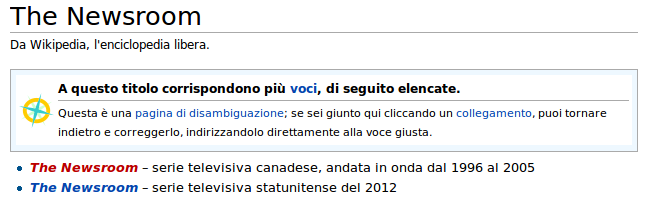
\includegraphics[width=12cm]{disambigua.png}
		\label{fig:tesi:stage:classificazione:disambiguazione}
		\caption{Pagina di disambiguazione \cite{wiki:disambigua}}
	\end{center}
\end{figure}

Occorre innanzi tutto rivedere la relazione uno-a-molti tra entità ed etichette, che diventa di tipo molti-a-molti e per cui vale la proprietà illustrata di seguito.

Siano $a_{j,k}$ e $a_{j,k'}$ accezioni distinte di un'etichetta $e_j$ e sia definita la funzione
\begin{equation}
f(a_{j,k}): A_j \rightarrow D
\end{equation}
che restituisce l'entità $d_i$ riferita dall'accezione $a_{j,k}$. Allora
\begin{equation}
a_{j,k} \neq a_{j,k'} \implies f(a_{j,k}) \neq f(a_{j,k'})
\end{equation}

L'equazione \ref{eq:tesi:stage:etichette-per-entità} conserva la propria validità, mentre la \ref{eq:tesi:stage:dizionario} dev'essere modificata per riflettere la differente molteplicità della suddetta relazione, ossia il fatto che ciascuna etichetta possa riferire una o più entità:
\begin{equation}
	\sum{\left|E_i\right|} = \sum{\left|B_i\right|} = \left|A\right| =	\sum{\left|A_j\right|} \geq \left|E\right| \:
	\footnote{La prima uguaglianza esprime una banale identità tra le etichette di un'entità e  e le accezioni corrispondenti; la seconda discende dal fatto che $P' = {B_1,B_2,\ldots}$ rappresenta una partizione di $A$ rispetto alle entità, mentre la successiva uguaglianza si deduce analogamente dal fatto che $P''={A_1, A_2, \ldots}$ è anch'essa partizione di $A$ (rispetto alle etichette); l'ultima disuguaglianza si deduce osservando che $\forall j \left|A_j\right| \geq 1$, ossia per ciascuna etichetta del dizionario esiste almeno un'accezione.}
\end{equation}

\begin{figure}[ht]
	\begin{center}
		
\includegraphics{placeholder.png}
		\caption{Accezioni di un'etichetta (+ modello relazionale)}
		\label{fig:tesi:stage:fase-uno:etichette-accezioni}
	\end{center}
\end{figure}

\pagebreak
Si registrano inoltre rilevanti ripercussioni in merito alla distinzione tra etichette primarie e secondarie. A ciascuna entità continuano ad essere associate una e una sola etichetta primaria, oltre ad un numero arbitrario (anche nullo) di etichette secondarie: ove ciascuna etichetta può riferirsi a diverse entità, tale distinzione varia a seconda dell'accezione considerata, poiché la medesima etichetta può essere primaria rispetto ad un entità e secondaria rispetto ad un'altra.

Per preservare i suddetti vincoli sulle relazioni tra etichette ed entità, si classificano le accezioni in \textsc{chiave} ($a_{j,0}$) o \textsc{sinonimiche} ($a_{j,1},\ldots,a_{j,\left|A_j\right|}$), a seconda che l'etichetta risulti rispettivamente primaria o secondaria per l'entità corrispondente. In questo modo si riesce a trasferire tale distinzione dalle etichette alle accezioni, preservando la percezione della relazione dal punto di vista dell'entità.

\begin{figure}[ht]
	\begin{center}
		
\includegraphics{placeholder.png}
		\caption{Accezioni chiave e sinonimiche (+ modello relazionale)}
		\label{fig:tesi:stage:classificazione:entita-etichette}
	\end{center}
\end{figure}

A risentire maggiormente dell'esistenza delle accezioni è il processo di ricerca di un'entità $d_i$ a partire da un'etichetta $e_j$: se $\left|A_j\right|\geq 2$ l'identificazione dell'entità richiede - da parte dell'utente - la selezione di un'accezione $a_{j,k} \in A_j$ tra le $\left|A_j\right|$ disponibili per indicare esplicitamente l'entità cui fa riferimento.

\subsection{Modello relazionale}

\begin{figure}[ht]
	\begin{center}
		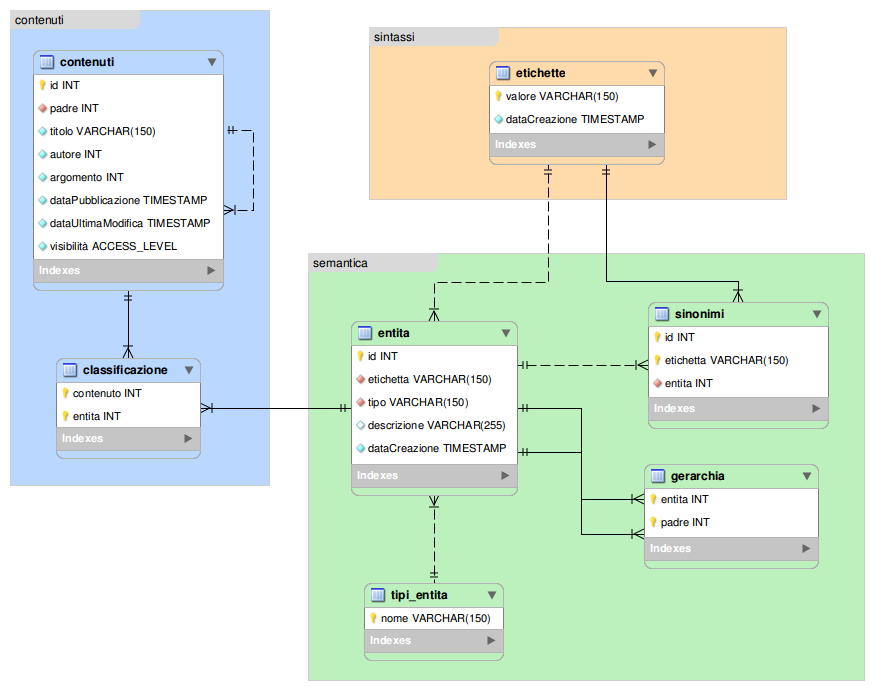
\includegraphics[width=14.7cm]{modello-er.png}
		\caption{Modello relazione del criterio di classificazione}
		\label{fig:tesi:stage:er:modello}
	\end{center}
\end{figure}

Al termine della fase progettuale, si rende necessario modificare il modello relazionale della piattaforma per integrare le informazioni addizionali legate al nuovo criterio di classificazione.

Rispetto all'immagine \ref{fig:tesi:stage:er:modello}, la sola tabella \textsf{contenuti} risulta importata dal modello relazionale della piattaforma per evidenziare alcune relazioni fondamentali. Le rimanenti sono organizzate in tre \textit{layer} (\textsf{contenuti}, \textsf{semantica} e \textsf{sintassi}) per chiarirne il ruolo all'interno del sistema di classificazione.

\paragraph{Etichette}
Le etichette sono rappresentate mediante la tabella \textsf{etichette} e sono identificate univocamente dalla stringa associata, che rappresenta l'attributo \textsf{etichette.valore}. Tale scelta risponde alla naturale identificazione dell'etichetta nella sequenza di caratteri corrispondente, costituisce una garanzia contro la presenza di duplicati e consente di recuperare il valore dell'etichetta primaria di un'entità senza dover effettuare un'operazione di \textit{join} tra le tabelle \textsf{entita} ed \textsf{etichette}.

\paragraph{Accezioni}
Le accezioni rappresentano un legame univoco tra le etichette e le entità e possono essere di tipo chiave o sinonimico. Esse non presentano attributi propri significativi, ma prevedono tre vincoli referenziali:
\begin{enumerate}
\item a ciascuna entità è associata una e una sola \textsc{accezione chiave} (relazione uno-a-uno), che identifica l'etichetta primaria;
\item a ciascuna entità sono associate $0\ldots n$ \textsc{accezioni sinonimiche} (relazione uno-a-molti), che rappresentano i sinonimi dell'etichetta primaria;
\item ciascuna etichetta possiede $0\ldots n$ \textsc{accezioni} (relazione uno-a-molti).
\end{enumerate}

\begin{figure}[ht]
	\begin{center}
		
\includegraphics{placeholder.png}
		\caption{Modello ad oggetti delle accezioni}
		\label{fig:tesi:stage:er:accezioni}
	\end{center}
\end{figure}

Ne consegue che sia la superclasse (\textsf{accezioni}) sia le sottoclassi (\textsf{accezioni\textunderscore chiave} e \textsf{accezioni\textunderscore sinonimiche}) presentano dei vincoli referenziali; in particolare, la presenza delle prime due relazioni costringe a distinguere - dal punto di vista dell'entità - tra accezioni chiave e sinonimiche.

Per modellare tale scenario vengono presi in considerazione tre possibili approcci:
\begin{description}
\item[Tabella unica] \hfill \\
La tabella unica ben si adatta a gestire l'assenza di attributi propri per le sottoclassi e ad esprimere i vincoli referenziali che coinvolgono la superclasse, ma non è in grado di esprimere e adeguatamente rappresentare quelli coinvolgenti le sottoclassi.
\item[Partizionamento orizzontale] \hfill \\
Il partizionamento orizzontale riesce a modellare i vincoli referenziali delle sottoclassi, ma non quello della superclasse, e genera due classi aventi i medesimi attributi.
\item[Partizionamento verticale] \hfill \\
Il partizionamento verticale consente di modellare correttamente tutti e tre i vincoli referenziali, relativi sia alla superclasse sia alle sottoclassi. Tuttavia si rende più complesso modificare il tipo di un'accezione e si introduce l'esigenza di un'operazione \textit{join} per recuperare la lista completa delle accezioni, pur non possedendo le sottoclassi attributi propri.
\end{description}

A seguito di alcune osservazioni si decide di adottare la soluzione della tabella unica:
\begin{itemize}
\item la distinzione tra etichette chiave e sinonimiche ha rilevanza essenzialmente dal punto di vista della classe \textsf{entita};
\item il vincolo referenziale tra \textsf{etichette} ed \textsf{accezioni} suggerisce che la distinzione di cui al punto precedente sia irrilevante dal punto di vista delle etichette, ragion per cui risulta utile mantenere tutte le accezioni nella medesima tabella.\footnote{Si consideri ad esempio il caso d'uso della ricerca di un'entità a partire da un'etichetta, ove occorre recuperare la lista completa delle relative accezioni.}
\item le sottoclassi non hanno attributi propri, per cui il partizionamento verticale e orizzontale sono ritenute soluzioni inadeguate.
\end{itemize}

Il soddisfacimento delle condizioni richieste viene raggiunto eliminando qualsiasi riferimento al tipo dell'accezione nella classe \textsf{accezioni} e modellando direttamente la relazione uno-a-uno tra le entità e le relative etichette primarie mediante una vincolo referenziale di chiave esterna nella classe \textsf{entita}, ossia \textsf{entita.etichetta}, che identifica la corrispondente etichetta primaria nella tabella \textsf{etichette}. Così facendo si riescono ad esprimere tutti i vincoli referenziali senza dover definire le sottoclassi.

%--------
% SECTION
%--------
\section{Interfaccia grafica}
\label{sec:tesi:stage:gui}
La seconda fase dell'attività di stage consiste nell'analisi e nella progettazione di un'interfaccia grafica per la consultazione dei risultati di ricerche sui contenuti informativi, che sfrutti il criterio di classificazione definito in precedenza e permetta all'utente di:
\begin{enumerate}
	\item impostare i parametri iniziali di ricerca, ossia le parole chiave e l'ambito;
	\item modificare a posteriori la lista delle entità cercate mediante sostituzione o eliminazione;
	\item filtrare i risultati di ricerca in accordo a criteri di classificazione o proprietà dei contenuti;
	\item consultare - in forma grafica o testuale - le proprietà fondamentali, i metadati di classificazione e i legami tra i contenuti;
	\item mostrare la discussione associata ad un contenuto informativo;
	\item impostare i filtri personalizzati (solo per utenti autenticati).
\end{enumerate}

Nella fase di progettazione dell'interfaccia grafica devono essere tenuti in debita considerazione alcuni requisiti di qualità desiderabili:
\begin{itemize}
  \item deve risultare intuitiva e facilmente utilizzabile da qualsiasi categoria di utenti, a prescindere dal livello di esperienza e dalla familiarità con piattaforme web esistenti (\textit{chat}, \textit{forum}, \textit{social network}, \ldots);
  \item dev'essere fruibile dal maggior numero possibile di dispositivi (\textit{computer}, \textit{tablet}, \textit{smartphone}, \ldots), ciascuno secondo le peculiari modalità di interazione;
  \item deve rappresentare in maniera ordinata ed efficace le informazioni, a prescindere dal numero di contenuti caricati.
\end{itemize}
 
\subsection{Filtri di ricerca}
\label{sec:tesi:stage:gui:filtri}
\paragraph{Requisiti}
La progettazione dei filtri di ricerca richiede innanzi tutto di scegliere i criteri di classificazione e le proprietà dei contenuti informativi (di seguito \textsc{parametri}) utilizzabili in combinazione ad un filtro: il requisito obbligatorio consiste nell'essere definiti su un insieme $U$ di possibili valori $u$, ciascuno dei quali - in un dato istante - dev'essere ammissibile ($u \in U_A$) o bloccato ($u \in U_B$). Deve quindi valere che $U_A \cap U_B = \emptyset$ e $U_A \cup U_B = U$.

Inizialmente tutti i valori relativi ad un certo parametro sono ammessi, ossia $U_a = U$ e $U_b = \emptyset$: l'azione dell'utente altera tale suddivisione dell'insieme $U$ bloccando un valore, autorizzandolo o azzerando il filtro, ossia rendendo ammissibili tutti i valori ($U_A = U$).

\paragraph{Soddisfacibilità}
Un contenuto informativo, incluso tra i risultati di ricerca, viene quindi visualizzato se e solo soddisfa tutti i parametri. A seconda che ciascun contenuto assuma un singolo valore (autore, data di pubblicazione, argomento, \ldots) o una lista (emozioni, etichette, intenzioni, \ldots), il parametro risulta soddisfatto se e solo se:
\begin{itemize}
\item il valore assunto è ammissibile (valore singolo);
\item almeno uno dei valori assunti è ammissibile (valori multipli).
\end{itemize}

\paragraph{Parametri}
Al termine dell'analisi viene redatta una lista completa dei parametri che soddisfano il requisito iniziale, visibile nella tabella \ref{tab:tesi:stage:parametri-filtri} (tra parentesi si riporta il nome della classe corrispondente, ove disponibile).\footnote{Il termine \textsc{etichette} riportato nella tabella designa in seguito il criterio di classificazione illustrato nella sezione \ref{sec:tesi:stage:criterio-classificazione}.}
\begin{table}[ht]
\centering
\begin{tabular}{|l|l|}
\hline
\textsc{Proprietà} & \textsc{Criteri di classificazione} \\ \hline
Autore (\textsf{User}) & Argomento (\textsf{Topic})\\
Data di pubblicazione & Emozioni (\textsf{Emotion}) \\
Tipo (\textsf{Type}) & Etichette (\textsf{Entity}) \\
Giudizi (\textsf{Rating}) & Interessi (\textsf{Interest}) \\
& Intenzioni (\textsf{Intention}) \\ \hline
\end{tabular}
\caption{Lista dei parametri per i filtri di ricerca}
\label{tab:tesi:stage:parametri-filtri}
\end{table}

\paragraph{Classificazione}
Per identificare i requisiti e i casi d'uso correlati ai filtri di ricerca conviene classificarli in relazione alla natura dell'insieme $U$ (ordinato, finito, \ldots) e alle possibili modalità d'interazione dell'utente (selezione di un intervallo di valori, impostazione di una soglia, \ldots), che determinano e alterano i sottoinsiemi $U_A$ e $U_B$. L'analisi si conclude con l'individuazione di quattro classi di filtri di ricerca:
\begin{description}
	\item[A lista di valori] \hfill \\
	Il filtro a lista di valori consente di autorizzare o bloccare selettivamente ciascun elemento dell'insieme $U$. I casi d'uso includono:
	\begin{itemize}
		\item la consultazione della lista dei valori ammessi;
		\item la consultazione della lista dei valori bloccati;
		\item l'autorizzazione di un valore;
		\item il blocco di un valore;
		\item l'azzeramento del filtro, equivalente all'autorizzazione di tutti i valori.
	\end{itemize}
	\item[A soglia di valore] \hfill \\
	Nel filtro a soglia di valore l'insieme $U$ è ordinato e rappresenta un intervallo caratterizzato da un minimo $min \in U$ ed un massimo $max \in U$. L'utente può scegliere arbitrariamente un valore $x$, purché soddisfi la condizione $min \leq x \leq max$; l'insieme dei valori soddisfacibili risulta così definito: $U_A = \lbrace u \in U : u \geq x \rbrace$.
	\item[Ad intervallo] \hfill \\
	Nel filtro ad intervallo l'insieme $U$ è ordinato e si caratterizza per un minimo $min \in U$ ed un massimo $max \in U$. L'utente è libero di selezionare l'estremo inferiore ($inf \in U$) e superiore ($sup\in U$) dell'intervallo, purché sia soddisfatta la seguente catena di disuguaglianze: $min \leq inf \leq sup \leq max$. L'insieme dei valori ammissibili risulta ovviamente $U_A = \lbrace u \in U : inf \leq u \leq sup \rbrace$. I casi d'uso annoverano:
	\begin{itemize}
		\item la selezione del valore minimo $inf$;
		\item la selezione del valore massimo $sup$.
		\item la selezione di un valore esatto ($inf = sup$).
	\end{itemize}
	\item[Ad interruttore] \hfill \\
	Il filtro ad interruttore consente all'utente di scegliere se applicare o meno ai risultati di ricerca il filtro corrispondente, che può essere di un tipo qualsiasi tra quelli descritti in precedenza. I casi d'uso prevedono solamente:
	\begin{itemize}
		\item l'attivazione del filtro;
		\item la disattivazione del filtro.
	\end{itemize}
\end{description}

\begin{table}[ht]
\centering
\begin{tabular}{|l|l|l|l|}
\hline
\textsc{Lista di valori} & \textsc{Soglia di valore} & \textsc{Intervallo} & \textsc{Interruttore}\\ \hline
Autore & Giudizi & Data di pubblicazione & Interessi \\
Argomento & & & \\
Emozioni & & & \\
Etichette & & & \\
Intenzioni & & & \\
Tipo & & & \\ \hline
\end{tabular}
\caption{Elenco dei parametri per i filtri di ricerca, suddisivi per tipo.}
\label{tab:tesi:stage:parametri-filtri-tipo}
\end{table}

\paragraph{Progettazione} La fase di progettazione deve integrare nell'architettura \underline{MVC} della piattaforma le classi e i parametri dei filtri di ricerca.
\begin{description}
  \item[Model] \hfill \\
  Ciascun tipo di filtro di ricerca è rappresentato dalla classe corrispondente nel package \textsf{model.filter}: \textsf{FList} (a lista di valori), \textsf{FRange} (ad intervallo), \textsf{FSwitch} (ad interruttore) ed \textsf{FValue} (a soglia di valore). Ciascuna di esse implementa un'interfaccia standard (\textsf{Filter}) per ridurre l'accoppiamento con le componenti del \textsc{controller} e facilitare l'estensibilità del sistema, ad esempio l'aggiunta di nuovi tipi di filtri.

\begin{figure}[ht]
	\begin{center}
		
\includegraphics{placeholder.png}
		\caption{Diagramma delle classi - Package \textit{model.filter}}
		\label{fig:tesi:stage:design:model-filter-classi}
	\end{center}
\end{figure}

  A parità di classe i parametri differiscono - dal punto di vista del filtro - per le specifiche dell'insieme $U$, in particolare per la sorgente (statica o dinamica) ed il tipo (emozioni, intenzioni, etichette, \ldots) di dati gestiti: ciascuna classe riportata nella tabella \ref{tab:tesi:stage:parametri-filtri} rappresenta - a livello di tipo - il corrispondente parametro per il filtro di ricerca (il generico insieme $U$) mentre - a livello di istanze - ciascuno dei possibili valori ($u \in U$).

	Per rendere le classi dei filtri polimorfe rispetto ai parametri, ossia per facilitarne l'aggiunta, l'aggiornamento e la rimozione, si definisce una classe astratta (\textsf{Metadata}), che tutte le suddette classi devono estendere. Essa include un metodo astratto (\textsf{getValueList}) da ridefinire per gestire opportunamente l'approvvigionamento dell'insieme dei valori $u \in U$, sia che si tratti di una lista statica (tipo, argomento, \ldots) o dinamica, ossia ricavata dai risultati di ricerca (autore, data di pubblicazione, \ldots): nel primo caso la lista di valori viene memorizzata nella classe come campo dati statico.

	I filtri vengono quindi creati a partire da una lista di valori, istanze di una sottoclasse concreta di \textsf{Metadata}: per favorire il disaccoppiamento si introduce una collezione di classi (\textsf{model.criteria}), che incapsulano tali valori e li rendono accessibili mediante un'interfaccia standard: \textsf{CList} (a lista di valori), \textsf{CRange} (ad intervallo) e \textsf{CValue} (a soglia di valore).

	Questa soluzione offre inoltre la possibilità di inizializzare un filtro ad interruttore con qualsiasi tipo di criterio, nascondendone così le specifiche alle classi che ne gestiscono solamente lo stato di attivazione (\textsf{FSwitch} e \textsf{FVSwitch}).

	\item[View] \hfill \\
	Ciascun tipo di filtro richiede un componente grafico differente, che metta a disposizione dell'utente gli strumenti e le opzioni adeguate per consentire un'interazione coerente rispetto a quanto previsto dai rispettivi casi d'uso: \textsf{FVList} (a lista di valori), \textsf{FVRange} (ad intervallo), \textsf{FVSwitch} (ad interruttore) e \textsf{FVValue} (a soglia di valore). Tali classi implementano la medesima interfaccia (\textsf{ViewFilter}) e devono essere inizializzate con un oggetto di tipo \textsf{Filter}.

	Al fine di assicurare che il tipo dinamico di questo oggetto sia coerente e consistente rispetto al tipo di componente grafico che stiamo costruendo (v. tabella \ref{tab:tesi:stage:design:filter-factory}) il costruttore di ciascuna classe considerata richiede un argomento avente tipo statico corrispondente ad una sottoclasse concreta di \textsf{Filter}, che rappresenta il filtro corrispondente.

	\item[Controller] \hfill \\
	Ciascun tipo di filtro prevede diverse modalità d'interazione, che richiedono di essere gestite mediante altrettante classi del \textit{package} \textsf{controller.filter}
\end{description}

\paragraph{Abstract Factory}
Per assicurare la corretta combinazione di istanze delle classi (v. tabella \ref{tab:tesi:stage:design:filter-factory}) si ricorre al \underline{design pattern} \textit{Abstract Factory}, che nasconde i dettagli relativi alle classi istanziate durante il processo di creazione di un filtro.

\begin{table}
	\centering
	\begin{tabular}{|l|c|c|c|c|c|}
	\hline
	 & \textsf{Metadata} & \textsf{Criterion} & \textsf{Filter} & \textsf{FilterController} & \textsf{FilterView} \\ \hline
	Argomento & \textsf{Topic} & \textsf{CList} & \textsf{FList} & \textsf{FCList} & \textsf{FVList} \\ \hline
	Autore & \textsf{User} & \textsf{CList} & \textsf{FList} & \textsf{FCList} & \textsf{FVList} \\ \hline
	Data di pubblicazione & \textsf{Date} & \textsf{CRange} & \textsf{FRange} & \textsf{FCRange}& \textsf{FVRange} \\ \hline
	Emozioni & \textsf{Emotion} & \textsf{CList} & \textsf{FList} & \textsf{FCList} & \textsf{FVList} \\ \hline
	Giudizi & \textsf{Rating} & \textsf{CValue} & \textsf{FValue} & \textsf{FCValue} & \textsf{FVValue} \\ \hline
	Intenzioni & \textsf{Intention} & \textsf{CList} & \textsf{FList} & \textsf{FCList} & \textsf{FVList} \\ \hline
	Interessi & \textsf{Interest} & \textsf{CList} & \textsf{FSwitch} & \textsf{FCSwitch} & \textsf{FVSwitch} \\ \hline
	Tipo & \textsf{Type} & \textsf{CList} & \textsf{FList} & \textsf{FCList} & \textsf{FVList} \\ \hline
	\end{tabular}
	\caption{Famiglie di prodotti}
	\label{tab:tesi:stage:design:filter-factory}
\end{table}

\subsection{Risultati di ricerca}
I risultati di una ricerca sono un insieme $S$ di contenuti informativi, all'interno del quale si individua un sottoinsieme $S_v \subseteq S$ formato da tutti e soli quelli visualizzati, che soddisfano cioé tutti i filtri di ricerca.

\paragraph{Contenuti visualizzati}
Per stabilire se un contenuto debba essere visualizzato ($s \in U_s$) occorre associargli dei metadati, che permettano di asserire se soddisfi tutti i fitri e - a fronte dell'interazione dell'utente con i filtri di ricerca - di aggiornare conseguentemente il sottoinsieme $S_v$.

Per tracciare qesta informazione si individuano due possibili soluzioni:
\begin{enumerate}
  \item un \textsc{contatore}, che tenga traccia del numero di filtri soddisfatti in un dato istante\footnote{Un contenuto viene visualizzato se e solo se il valore del contatore coincide con il numero di filtri attivi.};
  \item un'array di valori booleani, ciascuno dei quali esprima il soddisfacimento rispetto ad un singolo filtro attivo\footnote{Un contenuto viene visualizzato se e solo se tutti gli elementi sono veri.}.
\end{enumerate}

\paragraph{Aggiornamento di un filtro}
L'aggiornamento di un filtro da parte dell'utente presenta due principali fattori di differenziazione:
\begin{itemize}
\item la variazione di $S_v$, che esprime una diminuzione o un aumento dell'insieme dei valori ammissibili.
\item la classe del filtro, che determina l'esatta natura della condizione da verificare per asserire se un contenuto lo soddisfi o meno.
\end{itemize}

A seconda della variazione di $S_v$, per stabilire quali contenuti debbano essere visualizzati occorre:
\begin{itemize}
  \item $\Delta \left|S_v\right|<0$: individuare gli elementi $s \in S_v$ che non soddisfino la nuova condizione e spostarli in $S$;
  \item $\Delta \left|S_v\right|>0$: individuare gli elementi $s \in S$ che soddisfino il filtro corrente e spostare in $S_v$ quelli che li soddisfano tutti.
\end{itemize}

Nel primo caso, la soluzione del contatore consente un decremento unitario del valore corrispondente per tutti e soli gli elementi che non soddisfino il filtro, sapendo che la precondizione $s \in S_v$ implica il soddisfacimento di tutti i filtri, incluso quello corrente; nel secondo caso, invece, emerge un limite legato alla necessità di verificare il soddisfacimento del filtro nella condizione precedente e successiva all'aggiornamento dello stesso, non potendo stabilire sulla base del semplice valore del contatore se il filtro in questione fosse tra quelli soddisfatti o meno.

Vicevera, la soluzione con array di valori booleani offre un controllo granulare che consente - in entrambi i casi - di controllare solamente la postcondizione. 

\paragraph{Interazione con un filtro}
Ciascun tipo di filtro prevede diverse modalita d'interazione per modificare l'insieme dei valori ammissibili $S_v$:
\begin{itemize}
\item \textsc{A lista di valori}
\begin{itemize}
  \item Autorizzare un valore;
  \item bloccare un valore.
\end{itemize}
\item \textsc{A soglia di valore}
\begin{itemize}
  \item Aumentare il valore di soglia;
  \item diminuire il valore di soglia.
\end{itemize}
\item \textsc{Ad intervallo}
\begin{itemize}
  \item Aumentare il limite inferiore ($inf$);
  \item diminuire il limite inferiore ($inf$);
  \item aumentare il limite superiore ($sup$);
  \item diminuire il limite superiore ($sup$).
\end{itemize}
\item \textsc{Ad interruttore}
\begin{itemize}
  \item attivare il filtro;
  \item disattivare il filtro.
\end{itemize}
\end{itemize}

Per modellare tale scenario si ricorre al design pattern \textit{Command}, che consente di:
\begin{itemize}
  \item incapsulare le specifiche richieste di aggiornamento in oggetti di tipo \textsf{FilterUpdate};
  \item aggiungere nuovi comandi a fronte della definizione di nuovi tipi di filtri (\textsf{Filter});
  \item gestire le richieste concorrenti mediante una coda (\textsf{FilterUpdateQueue});
  \item processare serialmente le richieste grazie ad un \textit{dispatcher} (\textsf{FilterUpdateDispatcher}).
\end{itemize}

\begin{figure}[ht]
	\begin{center}
		
\includegraphics{placeholder.png}
		\caption{Diagramma delle classi per il design pattern \textit{Command}}
		\label{fig:tesi:stage:design:design-pattern-command}
	\end{center}
\end{figure}

Si conclude definendo un'opportuna gerarchia di classi \textsf{FilterUpdate}, che incapsulano la logica di controllo e le informazioni necessarie per aggiornare l'insieme $S_v$ a fronte della variazione di un filtro a causa di una specifica modalità d'interazione, tra quelle elencate in precedenza.

\subsection{Navigazione dei contenuti}
La componente di navigazione e consultazione dei risultati rappresenta un elemento cardine del prodotto poiché ha il compito di presentare all'utente i risultati di ricerca e le relative informazioni in modo chiaro e ordinato, a prescindere dal numero di contenuti e dalle specifiche del dispositivo utilizzato (dimensione, risoluzione dello schermo, modalità d'interazione, \ldots).

Seguendo un approccio \textit{bottom-up} ci si focalizza innanzi tutto sulla rappresentazione di un contenuto informativo (proprietà, metadati, relazioni) e in seguito sulla progettazione dell'interfaccia.

\paragraph{Contenuti}
Ciascun contenuto presenta numerose informazioni sotto forma di proprietà o metadati, questi ultimi legati a criteri di classificazione o contestuali alla ricerca.

Il primo passo consiste nel distinguere le informazioni \textsc{essenziali}, ossia utili o indispensabili all'identificazione e alla contestualizzazione di un contenuto, da quelle \textsc{aggiuntive} (o accessorie), che rappresentano un valore aggiunto a fronte di un particolare interesse dell'utente: le prime devono essere immediatamente e chiaramente riconoscibili e consultabili, mentre le seconde devono risultare nascoste ma facilmente accessibili.

\begin{table}
	\centering
	\begin{tabular}{|l|c|}
	\hline
	\textsc{Proprietà essenziali} & \textsc{Proprietà aggiuntive} \\ \hline
	Autore  & Argomento \\
	Attinenza & Emozioni\\
	Data di publicazione & Etichette \\
	Tipo & Giudizi \\
	Titolo & Intenzioni \\ \hline
	\end{tabular}
	\caption{Famiglie di prodotti}
	\label{tab:tesi:stage:design:tipi-proprietà}
\end{table}

Ciò consente di rendere più efficiente lo sfruttamento dello spazio disponibile comunicando all'utente le sole informazioni rilevanti per stabilire la pertinenza del contenuto: ove questo soddisfi le aspettative dell'utente, suscitandone l'interesse, egli può consultarne le informazioni aggiuntive.

Una volta compiuta tale distinzione occorre scegliere - per ciascuna informazione - la modalità di rappresentazione (grafica o testuale) più adatta per esprimerla e comunicarla all'utente, in modo da risultare intuitivamente comprensibile. Per soddisfare tali requisiti di qualità si fissano alcune linee guida:
\begin{itemize}
  \item mantenere un bilanciamento equilibrato tra informazioni testuali e grafiche, garantendo un adeguato livello di accessibilità; % (cite::WCAG)
  \item utilizzare in modo limitato e non esclusivo il colore;
  \item ricorrere a forme grafiche per esprimere informazioni quantitative o definite su un insieme limitato di valori, così da facilitare rispettivamente l'associazione tra la dimensione o il tipo di forma al corrispondente significato.
\end{itemize}
 
\begin{description}
\item[Argomento] \hfill \\
L'argomento di un contenuto è espresso sia in forma grafica, mediante l'uso del colore, sia testuale e viene collocato in posizione esterna rispetto alla forma per porre in risalto che si tratta di un'informazione aggiuntiva.
\item[Autore] \hfill \\
L'autore viene indicato in forma testuale.
\item[Attinenza] \hfill \\
Il grado di attinenza è espresso dalla dimensione proporzionale del componente grafico: in questo modo i contenuti maggiormente attinenti alla ricerca sono i primi a catturare l'attenzione dell'utente.
\item[Data di pubblicazione] \hfill \\
La data di pubblicazione è espressa in forma testuale.
\item[Emozioni] \hfill \\
Le emozioni associate ad un contenuto sono riportate in forma testuale.
\item[Etichette] \hfill \\
La lista delle entità assegnate al contenuto è riportata in forma testuale, con particolare evidenza e rilevanza visiva (ordine di apparizione, formato, \ldots) e semantica per quelle corrispondenti ai termini di ricerca.
\item[Giudizi] \hfill \\
I giudizi espressi dagli altri utenti sono riportati in forma testuale.
\item[Intenzioni] \hfill \\
Le intenzioni associate ad un contenuto sono riportate in forma testuale.
\item[Tipo] \hfill \\
Il tipo di contenuto è identificato dalla forma del componente grafico: la scelta di impiegare forme elementari risponde alla primeva esigenza di renderli immediatamente riconoscibili e comprensibili da qualsiasi categoria di utenti. La scelta della forma associata a ciascun tipo si avvale di analisi sociologiche svolte da altri membri del team di progetto.
\item[Titolo] \hfill \\
Il titolo è riportato in forma testuale.
\end{description}

Dal momento che la rappresentazione visiva di ciascuna classe di contenuti differisce essenzialmente per la forma elementare scelta, che a sua volta influenza il posizionamento ed il \textit{rendering} delle informazioni, si definisce una gerarchia di classi ove:
\begin{itemize}
  \item la classe base (\textsf{ContentView}) rappresenta il componente grafico di un generico contenuto (incluse le relative informazioni associate);
  \item le sottoclassi (\textsf{CVAnswer}, \textsf{CVEvent}, \ldots) identificano le singole classi di un contenuto, a ciascuna delle quali è associata la specifica forma elementare e un insieme di regole per la visualizzazione delle informazioni.
\end{itemize}
Questa scelta progettuale intende facilitare l'aggiornamento delle specifiche di \textit{rendering} di una classe di contenuti (variazione della forma o dell'organizzazione delle informazioni).

\begin{figure}[ht]
	\begin{center}
		
\includegraphics{placeholder.png}
		\caption{Diagramma delle classi del package \textit{view.content}}
		\label{fig:tesi:stage:design:view-content-classi}
	\end{center}
\end{figure}
 
\paragraph{Cronologia}
I risultati di una ricerca devono essere presentati secondo una struttura chiara ed ordinata, che ne agevoli la consultazione da parte dell'utente e che sia adeguatamente fruibile a prescindere dal numero di risultati o dal dispositivo utilizzato (risoluzione, dimensione dello schermo, modalità d'interazione, \ldots).

Per garantire la chiarezza espositiva e rappresentativa delle informazioni in scenari così differenti occorre tenere presente alcuni vincoli fisici, onde evitare un sovraccarico cognitivo dovuto all'eccessivo numero di risultati mostrati. Un fenomeno simile pregiudicherebbe radicalmente l'esperienza d'uso dell'interfaccia, rendendo assai difficoltoso individuare i contenuti d'interesse: date le previsioni di crescita della piattaforma, si ritiene opportuno includere sin da subito le potenziali criticità nelle valutazioni progettuali.

Una volta prese in considerazione alcune proposte di soluzione e vagliatine pro e contro, si giudica che l'organizzazione cronologica dei risultati di ricerca rappresenti una soluzione estremamente intuitiva dal punto di vista dell'utente e allo stesso tempo in grado di offrire un'eccellente flessibilità rispetto ai vincoli e limiti espressi in precedenza.

\paragraph{Raggruppamento}
Sia $[t_{min}, t_{max}]$ l'arco di tempo entro il quale sono stati pubblicati i risultati di ricerca. La soluzione individuata consiste nell'organizzare e suddividere i risultati di ricerca in \textsc{unità di tempo}, corrispndenti ad intervalli di lunghezza fissa (espressa in giorni, mesi o anni), gestendo opportunamente i seguenti parametri:
\begin{itemize}
  \item l'ampiezza della singola unità di tempo ($r$);
  \item il numero di unità di tempo visualizzate ($t$);
  \item il numero di contenuti visualizzati in ciascuna unità di tempo ($c$).
\end{itemize}

La variazione dinamica di tali parametri in base alle specifiche del dispositivo utilizzato consente di offrire un'esperienza di consultazione e navigazione dei risultati di ricerca su misura: è sufficiente definire alcune semplici regole o criteri che assegnino automaticamente dei valori ottimali in base ad opportune informazioni (risoluzione orizzontale o verticale, tipo di dispositivo, \ldots).

Ad esempio si potrebbe variare $t$ in maniera proporzionale alla risoluzione orizzontale dello schermo e $c$ rispetto alla risoluzione verticale, fissando rispettivamente dei valori costanti (in pixel) per la larghezza di un'unità di tempo e l'altezza di un contenuto. Il numero di risultati visualizzati corrisponderebbe sempre e comunque a:
\begin{equation}
c_{tot} = c * t
\end{equation}

Questo meccanismo consente di ottimizzare la visualizzazione delle unità di tempo (e i contenuti associati) a seconda dell'orientamento del dispositivo:
\begin{itemize}
  \item se orizzontale, le unità di tempo vengono mostrate come colonne affiancate e i risultati come un elenco verticale;
  \item se verticale, le unità di tempo possono essere mostrate come righe e i risultati come una lista di elementi;
\end{itemize}
%Gli strumenti e le opzioni di navigazione possono essere quindi adattati in modo da sfruttare al meglio lo spazio a disposizione.

Se si desidera visualizzare l'intero arco temporale $[t_{min}, t_{max}]$, ipotizzando che al fine di garantire una sufficiente leggibilità dei contenuti il numero di unità di tempo $t$ sia fissato, occorre impostare l'ampiezza $r$ delle unità di tempo in modo che:
\begin{equation}
 r = \frac{t_{max}-t_{min}}{t}
\end{equation}

In caso contrario, si mostrano solo i risultati relativi ad un sottointervallo di $[t_{min}, t_{max}]$, con un evidente guadagno in termini di:
\begin{itemize}
  \item efficienza legata alla possibilità di caricare i soli contenuti da visualizzare, ricorrendo per esempio ad un \underline{proxy};
  \item scalabilità rispetto al numero di contenuti e all'ampiezza dell'intervallo $[t_{min}, t_{max}]$.
\end{itemize}

Per ciascuna unità di tempo avente un numero di risultati di ricerca associati superiore al numero massimo di contenuti visualizzabili ($c_i > c$) potrebbe essere sufficiente includere un collegamento che consenta di visualizzare l'intera lista di risultati in uno spazio dedicato.

\paragraph{Ordinamento}
Particolarmente in questo caso scenario risulta opportuno definire uno o più criteri di ordinamento dei risultati all'interno di ciascuna unità temporale, cercando di favorire quelli aventi maggiore attinenza\footnote{Se $E_s$ è l'insieme delle etichette cercate e $E_c$ l'insieme delle etichette assegnate a ciascun contenuto si possono distinguere tre casi, a seconda del numero di etichette assegnate ad un contenuto tra quelle cercate: corrispondenza completa ($E_s \subseteq E_c$), parziale ($E_s \cap E_c \neq \emptyset$) o assente ($E_s \cap E_c = \emptyset$).}, pubblicati più di recente, \ldots .

La probabilità $P$ che un contenuto venga visualizzato in un'unità temporale è infatti inversamente proporzionale al numero di risultati ad essa associati:
\begin{equation}
P = \frac{c}{c_i}
\end{equation}

\paragraph{Navigazione}
Infine occorre fornire agli utenti gli strumenti e le opzioni di navigazione temporale dei contenuti per consentire loro di:
\begin{itemize}
  \item visualizzare i contenuti relativi al passato o al futuro (rispetto al periodo corrente);
  \item modificare la scala temporale, impostando un numero arbitrario di giorni, mesi o anni ($r$).
\end{itemize}

\begin{figure}[ht]
	\begin{center}
		
\includegraphics{placeholder.png}
		\caption{Asse temporale}
		\label{fig:tesi:stage:design:timeline}
	\end{center}
\end{figure}
